\section{La gestion de projet agile}

\paragraph{}
L'outil de gestion de projet est évidemment un point central de l'offre.
Il permet de suivre en détail le projet, de planifier les différentes étapes de l'évolution du logiciel, de suivre les changements dans le code et de rapporter des bugs.
Certains outils permettent même d'accéder à des fonctionnalités plus poussées comme la rédaction de documentation relative au projet, la gestion du temps passé sur chaque tâche, une gestion documentaire ou encore la planification de l'allocation de ressources.

\paragraph{}
La clé de l'outil de gestion de projet est le système de gestion des tâches, plus souvent dénommé \etranger{bugtracker}.

Chaque tâche est représentée par une entrée dans le système, appelée \textit{ticket}, \textit{demande} ou \textit{rapport de bug} selon les outils.
Elle dispose d'un titre et d'une description qui permettent de savoir en quoi elle consiste.
Elle possède également un statut dont le but est de préciser son état d'avancement : de façon minimaliste, le statut peut prendre les valeurs \og non réalisé \fg, \og en cours \fg{} et \og terminé \fg{} par exemple.
De plus, une tâche peut être attribuée à un utilisateur du système qui sera considéré comme la personne en charge de sa réalisation.
Une date d'échéance peut aussi être définie.
En outre, il existe souvent une fonctionnalité de commentaires qui permet aux utilisateurs de partager leur avis ou leur avancement.

Ainsi, le système de gestion des tâches est véritablement l'élément permet de suivre l'avancement du projet.
La granularité est plus ou moins fine en fonction du découpage en tâches qui est pratiqué.

\paragraph{}
Par ailleurs, il est possible d'utiliser un outil de gestion de projet agile pour suivre des tâches qui n'ont rien à voir avec celles d'un projet informatique.
Grâce à un système de gestion des tâches suffisamment généraliste et/ou personnalisé, il est possible de planifier des activités allant de l'organisation d'une réunion, le changement d'une ampoule en passant par la rédaction d'un rapport.

C'est avec ce type de problématique que les prestations de conseil deviennent deviennent incontournables.
Une bonne expérience et de bonnes connaissances sur les possibilités de l'outil permettent de segmenter efficacement les besoins de l'entreprise en entités et projets.
En effet, cela doit permettre aux utilisateurs finaux de mettre à profit le système de manière claire et efficace.

\begin{figure}
	\centering
	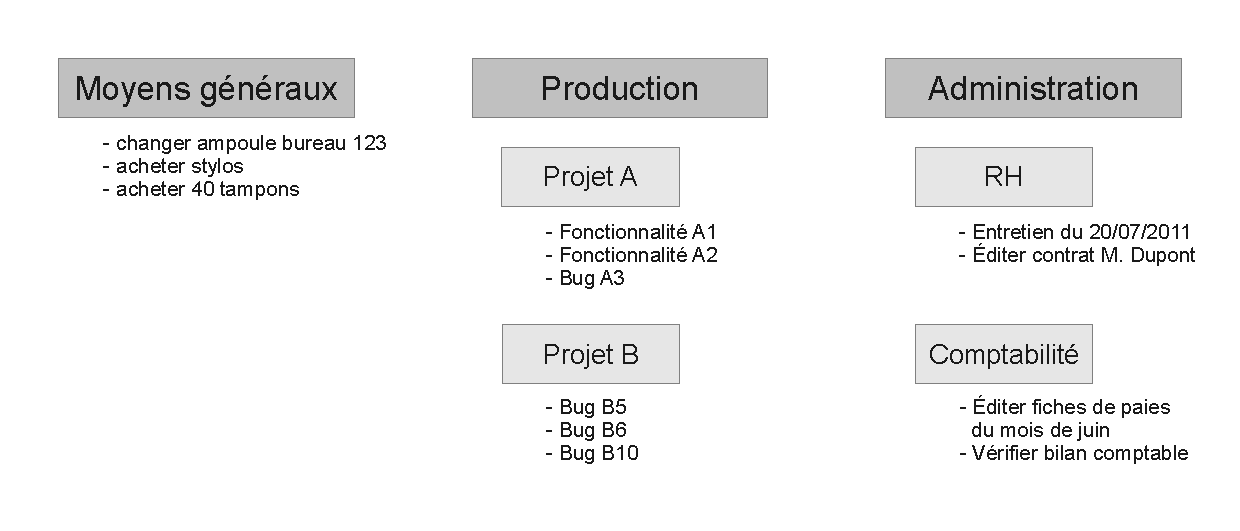
\includegraphics[width=13cm]{pic/taches}
	\caption{Exemple d'organisation d'un système de gestion de tâches pour une entreprise factice}
	\label{figure:pic-projet:taches}
\end{figure}

\paragraph{}
Un exemple de découpage des besoins d'une entreprise est représenté en \reffigure{pic-projet:taches}.

\paragraph{}
Finalement, ce type d'outil est complètement adapté à la gestion de projet agile.
Toutes les fonctionnalités qu'il intègre permettent une communication efficace de l'avancement du projet entre tous ses acteurs.
Aussi, sa facilité d'utilisation et les notifications des changements permettent d'accéder à une flexibilité maîtrisée.



\subsection{Outils}

\subsubsection{Redmine}

\paragraph{}
C'est le principal outil open source proposé par \asmile{} à ses clients.
Développé en Ruby avec le framework \aror, il a le gros avantage d'avoir une communauté très active.
Il s'utilise via le navigateur web.
Redmine est doté d'un bon nombre de fonctionnalités citées précédemment, parmi lesquelles :

\begin{itemize}
	\item une gestion en projets et sous-projets ;
	\item un système de gestion de tâches ;
	\item une vue des tâches sous la forme de GANTT ou de calendrier ;
	\item une gestion de feuilles de route\footnote{Dans le milieu informatique, ce terme est souvent utilisé (concurremment avec l'anglicisme \etranger{roadmap}) pour désigner le programme de développement d'un logiciel. Concrètement, on affecte les différentes tâches à réaliser à des jalons (ou versions). L'organisation et les priorités du développement apparaissent alors plus clairement.} ;
	\item un wiki\footnote{En informatique, un forum est un espace de discussion publique (ou au moins ouvert à plusieurs participants). Les discussions y sont archivées ce qui permet une communication asynchrone (c'est ce qui différencie les forums de la messagerie instantanée).~\cite{forum}} par projet ;
	\item un forum de discussion par projet ;
	\item un hébergement de fichiers et une gestion de documents par projet ;
	\item une intégration avec de nombreux systèmes de gestion de versions de code source (\cfsection{pic-source}) ;
	\item des notifications par e-mail ;
	\item une gestion fine des droits utilisateurs ;
	\item des groupes d'utilisateurs ;
	\item un support multilingue\ldots
\end{itemize}

De plus, Redmine est extensible par le biais de plugins.
Ainsi, de nombreuses fonctionnalités développées par la communauté peuvent être ajoutées, comme une gestion de budget ou une gestion de documents avancée par exemple.
Cela rend également possible le développement de fonctionnalités spécifiques pour répondre aux besoins pointus des clients.

Par ailleurs, \asmile{} propose également d'utiliser Redmine pour répondre à des besoins non-informatiques, comme évoqué précédemment.

\paragraph{}
Des captures d'écran de Redmine sont accessibles en \refannexe{redmine}.



\subsubsection{JIRA}

\paragraph{}
C'est un outil de gestion de projet similaire à Redmine du point de vue qu'il s'utilise par le biais d'une interface web.
Par contre, c'est un logiciel propriétaire développé en Java par Atlassian Software Systems.

Proposer un logiciel propriétaire n'est pas commun chez \asmile.
En fait il d'avère qu'il est complet et qu'il a beaucoup plu à Rexel, un des clients de \asmile{} qui a commandé l'intégration des autres outils open source de l'offre.

Son atout le plus notable est l'ensemble des représentations graphiques qu'il propose, mettant en relief les données des différents projets suivis.

\paragraph{}
Des captures d'écran de JIRA sont accessibles en \refannexe{jira}.



\subsection{Missions}

\subsubsection{Formation JIRA chez Rexel}

J'ai eu l'occasion de participer au début de mon stage à la formation JIRA donnée chez Rexel par mon maître de stage \agulet.
J'ai pu ainsi découvrir le produit, ses fonctionnalités et ses possibilités.



\subsubsection{Développement Redmine pour RAGT}

\paragraph{}
Pendant mon stage, \agulet{} a effectué une mission dans l'entreprise RAGT qui a commandé une mise en place complète de l'outil Redmine ainsi qu'une prestation de conseil.
Confronté à des problématiques spécifiques, il m'a demandé d'ajouter de nouvelles fonctionnalités au système de gestion de projets.

À cette occasion, j'ai appris à développer en langage Ruby et je me suis confronté à la documentation du framework \aror{} et à celle de Redmine.

\paragraph{}
Le premier développement a consisté à améliorer le système de gestion de tâches existant.
Dans Redmine, il est possible de lier des tâches entre elles en précisant le type de lien (\og lié à \fg, \og précède \fg, \og suit \fg, \og bloque \fg\ldots).
Ainsi, j'ai apporté la possibilité de créer à la volée une tâche à lier à une tâche existante.

\paragraph{}
Pour le second développement, j'ai amélioré un plugin existant : Better GANTT Chart.
Celui-ci améliore les graphes GANTT des tâches en ajoutant des flèches pour représenter les dépendances inter-tâches, issues des liens décrits précédemment.

Or, dans Redmine, il est possible de lier une tâche d'un projet à celle d'un autre projet.
Le problème est que les tâches issues d'un projet différent ne sont pas dessinées sur le GANTT. 
Je me suis alors chargé d'ajouter cette fonctionnalité que l'équipe à l'origine du plugin s'est empressée d'intégrer dans leur base de code.

\paragraph{}
Enfin, le dernier développement a concerné la possibilité de mettre en place des sous-groupes d'utilisateurs.
En effet, les groupes regroupent des utilisateurs de façon à les associer en masse à un projet donné.
Mettre en place des sous-groupes consiste à inclure des groupes dans un autre : de cette façon il est possible de construire une organisation complexe en évitant de répéter des affectations. 

Cette fois, j'ai développé directement dans le c\oe ur de Redmine et j'ai soumis la fonctionnalité à l'équipe qui dirige le développement.
Malheureusement, rien n'a pu être intégré pour l'instant faute de réponse.

